% Options for packages loaded elsewhere
\PassOptionsToPackage{unicode}{hyperref}
\PassOptionsToPackage{hyphens}{url}
\PassOptionsToPackage{dvipsnames,svgnames,x11names}{xcolor}
%
\documentclass[
]{report}

\usepackage{amsmath,amssymb}
\usepackage{setspace}
\usepackage{iftex}
\ifPDFTeX
  \usepackage[T1]{fontenc}
  \usepackage[utf8]{inputenc}
  \usepackage{textcomp} % provide euro and other symbols
\else % if luatex or xetex
  \usepackage{unicode-math}
  \defaultfontfeatures{Scale=MatchLowercase}
  \defaultfontfeatures[\rmfamily]{Ligatures=TeX,Scale=1}
\fi
\usepackage{lmodern}
\ifPDFTeX\else  
    % xetex/luatex font selection
\fi
% Use upquote if available, for straight quotes in verbatim environments
\IfFileExists{upquote.sty}{\usepackage{upquote}}{}
\IfFileExists{microtype.sty}{% use microtype if available
  \usepackage[]{microtype}
  \UseMicrotypeSet[protrusion]{basicmath} % disable protrusion for tt fonts
}{}
\makeatletter
\@ifundefined{KOMAClassName}{% if non-KOMA class
  \IfFileExists{parskip.sty}{%
    \usepackage{parskip}
  }{% else
    \setlength{\parindent}{0pt}
    \setlength{\parskip}{6pt plus 2pt minus 1pt}}
}{% if KOMA class
  \KOMAoptions{parskip=half}}
\makeatother
\usepackage{xcolor}
\usepackage[top=30mm,left=20mm,heightrounded]{geometry}
\setlength{\emergencystretch}{3em} % prevent overfull lines
\setcounter{secnumdepth}{-\maxdimen} % remove section numbering
% Make \paragraph and \subparagraph free-standing
\makeatletter
\ifx\paragraph\undefined\else
  \let\oldparagraph\paragraph
  \renewcommand{\paragraph}{
    \@ifstar
      \xxxParagraphStar
      \xxxParagraphNoStar
  }
  \newcommand{\xxxParagraphStar}[1]{\oldparagraph*{#1}\mbox{}}
  \newcommand{\xxxParagraphNoStar}[1]{\oldparagraph{#1}\mbox{}}
\fi
\ifx\subparagraph\undefined\else
  \let\oldsubparagraph\subparagraph
  \renewcommand{\subparagraph}{
    \@ifstar
      \xxxSubParagraphStar
      \xxxSubParagraphNoStar
  }
  \newcommand{\xxxSubParagraphStar}[1]{\oldsubparagraph*{#1}\mbox{}}
  \newcommand{\xxxSubParagraphNoStar}[1]{\oldsubparagraph{#1}\mbox{}}
\fi
\makeatother


\providecommand{\tightlist}{%
  \setlength{\itemsep}{0pt}\setlength{\parskip}{0pt}}\usepackage{longtable,booktabs,array}
\usepackage{calc} % for calculating minipage widths
% Correct order of tables after \paragraph or \subparagraph
\usepackage{etoolbox}
\makeatletter
\patchcmd\longtable{\par}{\if@noskipsec\mbox{}\fi\par}{}{}
\makeatother
% Allow footnotes in longtable head/foot
\IfFileExists{footnotehyper.sty}{\usepackage{footnotehyper}}{\usepackage{footnote}}
\makesavenoteenv{longtable}
\usepackage{graphicx}
\makeatletter
\def\maxwidth{\ifdim\Gin@nat@width>\linewidth\linewidth\else\Gin@nat@width\fi}
\def\maxheight{\ifdim\Gin@nat@height>\textheight\textheight\else\Gin@nat@height\fi}
\makeatother
% Scale images if necessary, so that they will not overflow the page
% margins by default, and it is still possible to overwrite the defaults
% using explicit options in \includegraphics[width, height, ...]{}
\setkeys{Gin}{width=\maxwidth,height=\maxheight,keepaspectratio}
% Set default figure placement to htbp
\makeatletter
\def\fps@figure{htbp}
\makeatother

\usepackage{fancyhdr}
  \pagestyle{fancy}
  \fancyhead[C]{UOC}
  \fancyhead[R]{aperez-b@uoc.edu}
  \fancyfoot{}
  \fancyfoot[C]{\thepage}
\usepackage{fvextra}
\DefineVerbatimEnvironment{Highlighting}{Verbatim}{breaklines,commandchars=\\\{\}}
\DefineVerbatimEnvironment{OutputCode}{Verbatim}{breaklines,commandchars=\\\{\}}
\makeatletter
\@ifpackageloaded{tcolorbox}{}{\usepackage[skins,breakable]{tcolorbox}}
\@ifpackageloaded{fontawesome5}{}{\usepackage{fontawesome5}}
\definecolor{quarto-callout-color}{HTML}{909090}
\definecolor{quarto-callout-note-color}{HTML}{0758E5}
\definecolor{quarto-callout-important-color}{HTML}{CC1914}
\definecolor{quarto-callout-warning-color}{HTML}{EB9113}
\definecolor{quarto-callout-tip-color}{HTML}{00A047}
\definecolor{quarto-callout-caution-color}{HTML}{FC5300}
\definecolor{quarto-callout-color-frame}{HTML}{acacac}
\definecolor{quarto-callout-note-color-frame}{HTML}{4582ec}
\definecolor{quarto-callout-important-color-frame}{HTML}{d9534f}
\definecolor{quarto-callout-warning-color-frame}{HTML}{f0ad4e}
\definecolor{quarto-callout-tip-color-frame}{HTML}{02b875}
\definecolor{quarto-callout-caution-color-frame}{HTML}{fd7e14}
\makeatother
\makeatletter
\@ifpackageloaded{caption}{}{\usepackage{caption}}
\AtBeginDocument{%
\ifdefined\contentsname
  \renewcommand*\contentsname{Table of contents}
\else
  \newcommand\contentsname{Table of contents}
\fi
\ifdefined\listfigurename
  \renewcommand*\listfigurename{List of Figures}
\else
  \newcommand\listfigurename{List of Figures}
\fi
\ifdefined\listtablename
  \renewcommand*\listtablename{List of Tables}
\else
  \newcommand\listtablename{List of Tables}
\fi
\ifdefined\figurename
  \renewcommand*\figurename{Figure}
\else
  \newcommand\figurename{Figure}
\fi
\ifdefined\tablename
  \renewcommand*\tablename{Table}
\else
  \newcommand\tablename{Table}
\fi
}
\@ifpackageloaded{float}{}{\usepackage{float}}
\floatstyle{ruled}
\@ifundefined{c@chapter}{\newfloat{codelisting}{h}{lop}}{\newfloat{codelisting}{h}{lop}[chapter]}
\floatname{codelisting}{Listing}
\newcommand*\listoflistings{\listof{codelisting}{List of Listings}}
\makeatother
\makeatletter
\makeatother
\makeatletter
\@ifpackageloaded{caption}{}{\usepackage{caption}}
\@ifpackageloaded{subcaption}{}{\usepackage{subcaption}}
\makeatother

\ifLuaTeX
  \usepackage{selnolig}  % disable illegal ligatures
\fi
\usepackage{bookmark}

\IfFileExists{xurl.sty}{\usepackage{xurl}}{} % add URL line breaks if available
\urlstyle{same} % disable monospaced font for URLs
\hypersetup{
  pdftitle={CA 2},
  pdfauthor={Alejandro Pérez Bueno},
  colorlinks=true,
  linkcolor={blue},
  filecolor={Maroon},
  citecolor={Blue},
  urlcolor={Blue},
  pdfcreator={LaTeX via pandoc}}


\title{CA 2}
\usepackage{etoolbox}
\makeatletter
\providecommand{\subtitle}[1]{% add subtitle to \maketitle
  \apptocmd{\@title}{\par {\large #1 \par}}{}{}
}
\makeatother
\subtitle{E-Commerce}
\author{Alejandro Pérez Bueno}
\date{Nov 14, 2024}

\begin{document}
\maketitle

\renewcommand*\contentsname{Table of Contents}
{
\hypersetup{linkcolor=}
\setcounter{tocdepth}{2}
\tableofcontents
}

\setstretch{1.25}
\newpage{}

\section{Exercise 1}\label{exercise-1}

\subsection{a)}\label{a}

\subsubsection{\texorpdfstring{\textbf{New
Entities}}{New Entities}}\label{new-entities}

\begin{itemize}
\item
  \textbf{SUPPLIER}: This entity would store information about the new
  product suppliers.

  \begin{itemize}
  \item
    Attributes: \texttt{supplier\_id} (primary key),
    \texttt{supplier\_name}, \texttt{contact\_person}, \texttt{email},
    \texttt{phone}, \texttt{address}.

    \begin{itemize}
    \tightlist
    \item
      Data manipulation operations:

      \begin{itemize}
      \tightlist
      \item
        \texttt{add\_supplier}: Inserts a new supplier into the SUPPLIER
        table.
      \item
        \texttt{modify\_supplier}: Updates supplier information in the
        SUPPLIER table.
      \item
        \texttt{delist\_supplier}: Logically removes a supplier from the
        SUPPLIER table.
      \end{itemize}
    \end{itemize}
  \end{itemize}
\item
  \textbf{PREMIUM\_CUSTOMER}: This entity represents customers who have
  signed up for the premium program. It would be a specialized entity
  inheriting from the CUSTOMER entity.

  \begin{itemize}
  \item
    Attributes: \texttt{customer\_id} (primary key, foreign key
    referencing CUSTOMER), \texttt{points\_balance}.

    \begin{itemize}
    \item
      Data manipulation operations:

      \begin{itemize}
      \tightlist
      \item
        \texttt{register\_premium\_customer}: Creates a new
        PREMIUM\_CUSTOMER record when a customer enrolls in the premium
        program. This operation should also add the customer to the
        CUSTOMER table if they are not already registered.
      \item
        \texttt{update\_points}: Updates the \texttt{points\_balance}
        for a PREMIUM\_CUSTOMER after a purchase.
      \item
        \texttt{redeem\_points}: Allows a PREMIUM\_CUSTOMER to redeem
        points for discounts or other rewards.
      \item
        \texttt{cancel\_premium\_customer}: Removes a customer from the
        PREMIUM\_CUSTOMER table when they cancel their premium
        membership.
      \end{itemize}
    \end{itemize}
  \end{itemize}
\item
  \textbf{PROMOTION}: This entity stores information about the various
  promotions being offered.

  \begin{itemize}
  \item
    Attributes: \texttt{promotion\_id} (primary key),
    \texttt{promotion\_name}, \texttt{start\_date}, \texttt{end\_date},
    \texttt{description}.

    \begin{itemize}
    \item
      Data manipulation operations:

      \begin{itemize}
      \tightlist
      \item
        \texttt{add\_promotion}: Adds a new promotion to the PROMOTION
        table.
      \item
        \texttt{modify\_promotion}: Updates the details of an existing
        promotion.
      \item
        \texttt{remove\_promotion}: Deletes a promotion from the
        PROMOTION table.
      \end{itemize}
    \end{itemize}
  \end{itemize}
\end{itemize}

\subsubsection{\texorpdfstring{\textbf{New
Relationships}}{New Relationships}}\label{new-relationships}

\begin{itemize}
\item
  \textbf{SUPPLIES}: This relationship connects the SUPPLIER entity to
  the PRODUCT entity. It represents which suppliers provide which
  products. This relationship is M-N because a supplier can supply
  multiple products, and a product can be supplied by multiple
  suppliers.

  \begin{itemize}
  \item
    Attributes: None.

    \begin{itemize}
    \tightlist
    \item
      Data manipulation operations: No specific operations are required,
      as this relationship is managed by the operations that add and
      remove products from the catalogue.
    \end{itemize}
  \end{itemize}
\item
  \textbf{INCLUDED\_IN}: This relationship connects the PRODUCT entity
  to the PROMOTION entity. This relationship is M-N because a product
  can be part of multiple promotions, and a promotion can include
  multiple products.

  \begin{itemize}
  \item
    Attributes: \texttt{quantity} (the number of units of the product
    required to qualify for the promotion), \texttt{free\_product\_id}
    (foreign key referencing PRODUCT, if applicable). This attribute
    would store the ID of the product offered for free in a ``buy X, get
    Y free'' promotion.

    \begin{itemize}
    \item
      Data manipulation operations:

      \begin{itemize}
      \tightlist
      \item
        \texttt{add\_product\_to\_promotion}: Adds a product to a
        promotion.
      \item
        \texttt{remove\_product\_from\_promotion}: Removes a product
        from a promotion.
      \end{itemize}
    \end{itemize}
  \end{itemize}
\end{itemize}

\subsubsection{\texorpdfstring{\textbf{Modifications to Existing
Operations}}{Modifications to Existing Operations}}\label{modifications-to-existing-operations}

\begin{itemize}
\item
  \textbf{\texttt{list\_product}}: This operation would need to be
  modified to include the \texttt{supplier\_id} as an input parameter.
  This ensures that newly added products are associated with their
  corresponding supplier.
\item
  \textbf{\texttt{calculate\_order\_total}}: This operation needs
  modification to factor in discounts offered to PREMIUM\_CUSTOMERs and
  promotional discounts based on the \texttt{INCLUDED\_IN} relationship.
\end{itemize}

\subsubsection{\texorpdfstring{\textbf{New
Operations}}{New Operations}}\label{new-operations}

\begin{itemize}
\tightlist
\item
  \textbf{\texttt{apply\_promotion}}: This operation would be executed
  during the checkout process to check if any promotions apply to the
  customer's order and adjust the order total accordingly.
\end{itemize}

These modifications enhance the existing conceptual model by allowing
for:

\begin{itemize}
\tightlist
\item
  \textbf{Supplier management}: The addition of the SUPPLIER entity
  allows the toy company to manage its supplier network efficiently.
\item
  \textbf{Promotion creation and management}: The toy company can define
  various types of promotions and associate them with specific products.
\item
  \textbf{Premium customer management}: The toy company can track
  PREMIUM\_CUSTOMERs and their points balance, enabling personalized
  offers and rewards.
\end{itemize}

\begin{tcolorbox}[enhanced jigsaw, coltitle=black, leftrule=.75mm, colframe=quarto-callout-note-color-frame, title=\textcolor{quarto-callout-note-color}{\faInfo}\hspace{0.5em}{Note}, titlerule=0mm, arc=.35mm, colbacktitle=quarto-callout-note-color!10!white, colback=white, left=2mm, toprule=.15mm, bottomrule=.15mm, toptitle=1mm, breakable, bottomtitle=1mm, rightrule=.15mm, opacityback=0, opacitybacktitle=0.6]

The data manipulation operations associated with each new entity and
relationship ensure data integrity and consistency. The modifications to
existing operations and the creation of new operations support the new
functionalities and integrate them seamlessly with the existing system.

\end{tcolorbox}

\subsection{b)}\label{b}

The image positions technology and marketing as integral components of
gamification. When applied to an online store's promotion system, both
elements play critical roles in implementation.

\textbf{Technology} underpins the entire gamified promotion system.
\textbf{Screaming Frog SEO Spider} is a software tool that can analyze
various aspects of a website, including page titles, meta descriptions,
and internal linking. It helps identify technical SEO issues and
provides data that can be used for optimization. These technical
capabilities are essential for implementing gamified elements like point
tracking, leaderboards, and achievement badges. A robust database, as
discussed in our previous conversation and exemplified in source, is
crucial for storing and managing the data generated by customer
interactions within the gamified system.

\textbf{Marketing} leverages technology to create engaging and effective
promotional campaigns. Marketing strategies in e-commerce rely heavily
on data analysis and customer relationship management (CRM). A data
warehouse, described in source, serves as a repository of historical
data from various sources, including the operational database, which can
be used for analyzing customer behavior and preferences. This data
empowers marketing teams to design gamified promotions tailored to
specific customer segments, driving engagement and encouraging desired
actions. For example, Screaming Frog SEO Spider can be used to track the
performance of different landing pages and identify areas for
improvement, which can inform the design of gamified elements within
those pages.

\section{Exercise 2}\label{exercise-2}

\subsection{a)}\label{a-1}

\textbf{SEO} (Search Engine Optimization) is the practice of optimizing
a website to improve its visibility in organic search engine results,
while \textbf{SEM} (Search Engine Marketing) is a broader term that
encompasses both SEO and paid search advertising strategies, such as
Pay-Per-Click (PPC) campaigns. Here are some differences among the two
found on the internet:

\begin{itemize}
\item
  \textbf{Cost}: SEO is generally cost-effective over time, focusing on
  organic strategies, while SEM involves ongoing costs for paid
  advertising.
\item
  \textbf{Speed}: SEO takes time to show results, often months, whereas
  SEM can provide immediate visibility through paid ads.
\item
  \textbf{Sustainability}: SEO offers long-term, sustainable traffic
  growth, while SEM traffic stops when ad spending ceases.
\item
  \textbf{Components}: SEO focuses on optimizing for organic search
  results, while SEM includes both SEO and paid search strategies like
  PPC.
\item
  \textbf{Goal}: SEO aims to improve organic rankings, while SEM seeks
  to increase visibility through both organic and paid methods.
\item
  \href{https://wegic.ai/blog/seo-vs-sem-key-differences.html}{SEO vs
  SEM: Key Differences}
\item
  \href{https://www.linkedin.com/pulse/whats-difference-between-seo-sem-intellezy-lvxkc}{What's
  The Difference Between SEO and SEM?}
\end{itemize}

\subsection{b)}\label{b-1}

\subsubsection{Link Building}\label{link-building}

Link building is crucial for establishing authority and trustworthiness.
In e-commerce, acquiring high-quality backlinks from reputable sites
signals to search engines that your site is credible. Techniques include
guest blogging, influencer partnerships, and creating shareable content.
Quality over quantity is essential, as links from authoritative sites
carry more weight and can significantly boost search rankings.

\subsubsection{Social Media Engagement}\label{social-media-engagement}

Active social media presence enhances brand visibility and drives
traffic to your e-commerce site. Sharing engaging content, interacting
with followers, and leveraging platforms like Instagram and Pinterest
can increase brand awareness and generate backlinks. While social
signals aren't direct ranking factors, they contribute to overall online
presence and can indirectly influence SEO by driving traffic and
engagement.

\subsubsection{Online Reviews and Reputation
Management}\label{online-reviews-and-reputation-management}

Positive reviews and a strong online reputation build trust with
potential customers and search engines. Encourage satisfied customers to
leave reviews on platforms like Google My Business and Yelp. Responding
to reviews, both positive and negative, shows engagement and can improve
customer perception. A strong reputation can lead to increased
click-through rates and conversions, positively impacting search
rankings.

\begin{itemize}
\tightlist
\item
  \href{https://blog.bluetuskr.com/on-page-and-off-page-seo-ecommerce}{Understanding
  On-Page and Off-Page E-commerce SEO}
\item
  \href{https://www.semrush.com/blog/off-page-seo/}{What Is Off-Page
  SEO?}
\end{itemize}

\subsection{c)}\label{c}

I have run \emph{Screaming Frog} on the site
\href{https://uoc.edu}{uoc.edu}, as seen on these images:

\begin{figure}[H]

{\centering 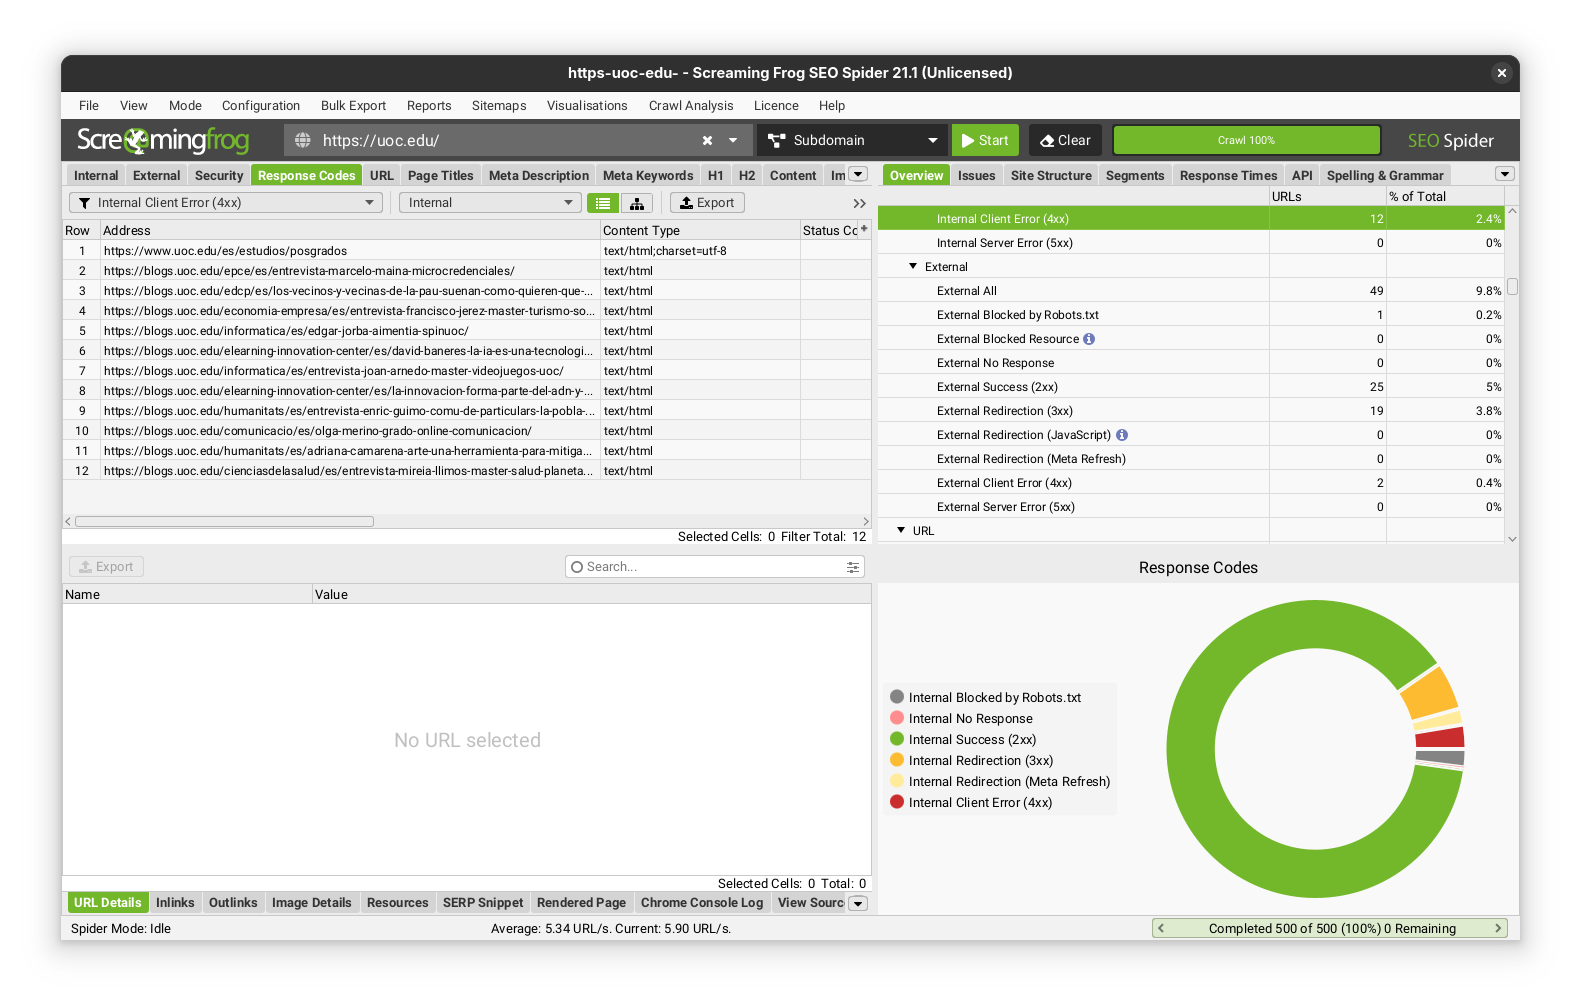
\includegraphics{./img/frog.png}

}

\caption{Test results}

\end{figure}%%
\begin{figure}[H]

{\centering 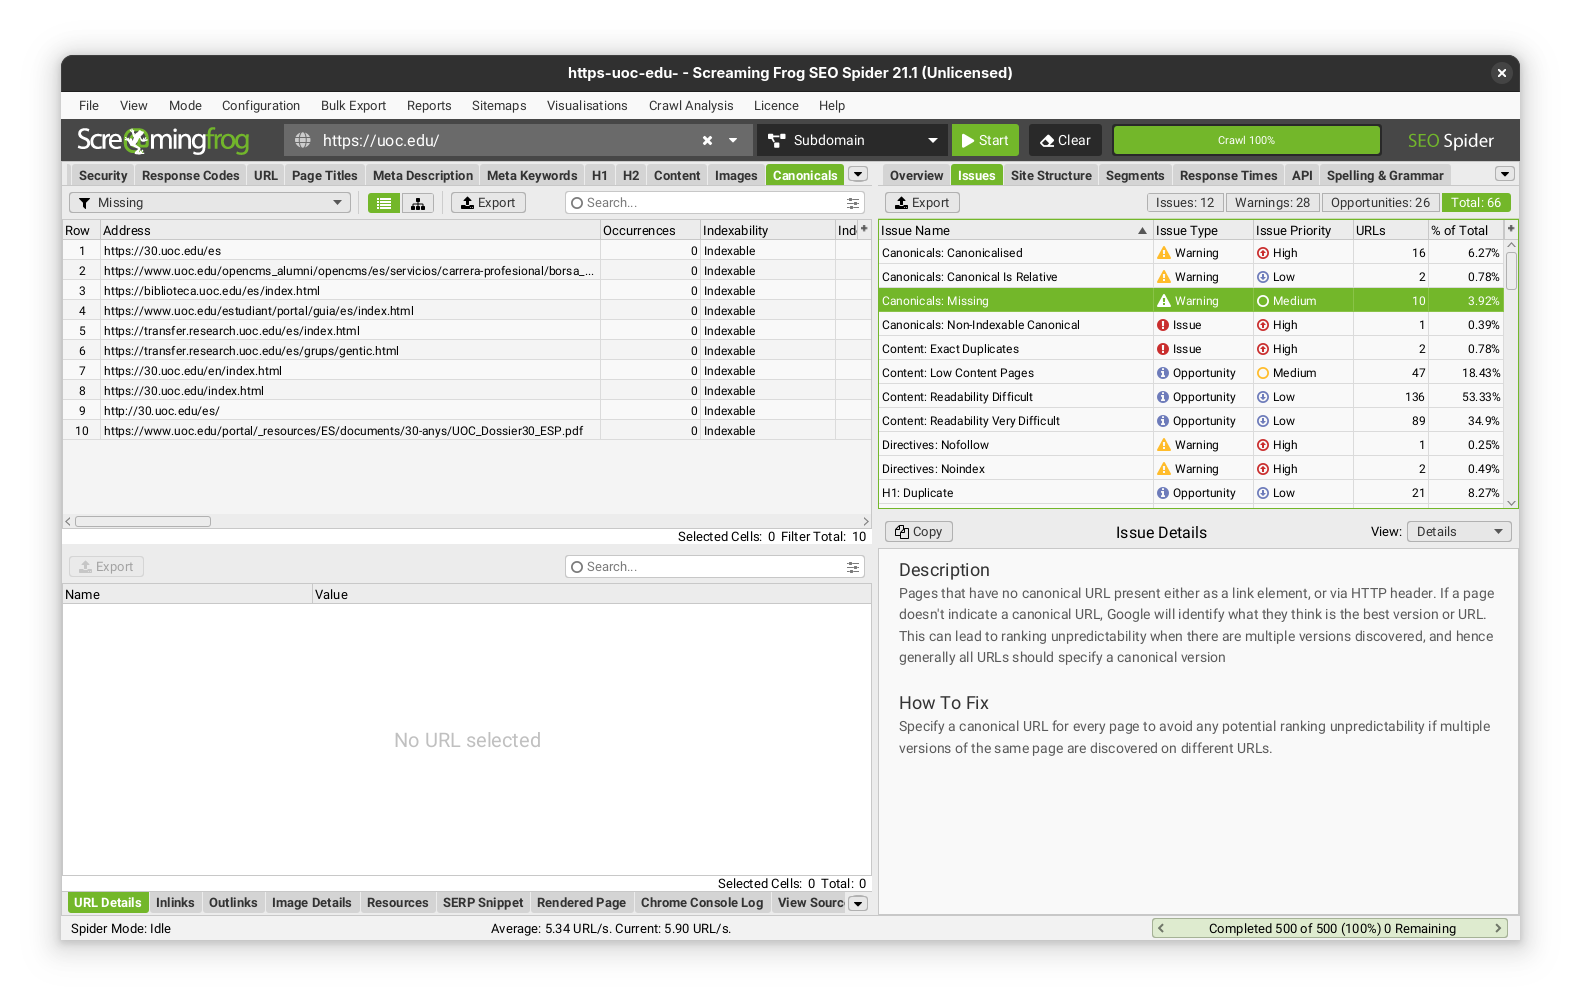
\includegraphics{./img/error.png}

}

\caption{Test errors and warnings}

\end{figure}%

Here are the three issues found and my proposed solutions to each of
them:

\begin{enumerate}
\def\labelenumi{\arabic{enumi}.}
\tightlist
\item
  \textbf{Non-Indexable Canonical:}

  \begin{itemize}
  \tightlist
  \item
    \textbf{Description:} This issue occurs when a page has a canonical
    URL that is non-indexable, meaning it might be blocked by
    \texttt{robots.txt}, have no response, or return errors. This can
    confuse search engines and lead to indexing issues.
  \item
    \textbf{Fix:} Ensure that canonical URLs point to indexable pages by
    checking for any blocks in \texttt{robots.txt}, resolving any server
    errors, and ensuring the canonical page is not set to ``noindex.''
  \end{itemize}
\item
  \textbf{Missing Canonicals:}

  \begin{itemize}
  \tightlist
  \item
    \textbf{Description:} Pages without a canonical URL can lead to
    ranking unpredictability, as search engines may not know which
    version of a page to prioritize.
  \item
    \textbf{Fix:} Specify a canonical URL for each page to guide search
    engines in identifying the preferred version, especially when
    multiple versions of a page exist.
  \end{itemize}
\item
  \textbf{Exact Duplicates:}

  \begin{itemize}
  \tightlist
  \item
    \textbf{Description:} Identical pages can split PageRank signals and
    cause unpredictability in search rankings. This happens when
    multiple URLs serve the same content.
  \item
    \textbf{Fix:} Implement a single canonical version for each set of
    duplicate pages and use 301 redirects to point other versions to
    this canonical URL, ensuring internal links also point to the
    canonical version.
  \end{itemize}
\end{enumerate}




\end{document}
